\documentclass{beamer}
\usetheme{cupertino}
\usepackage{amsmath} % formule matematice
\usepackage[noend]{algorithmic}
\usepackage{algorithm}

\setbeamertemplate{footline}[frame number]
%\usepackage{beamerthemesplit}
%\usetheme{classic} %\usetheme{Boadilla} %\usetheme{shadow}
\definecolor{gray}{rgb}{0.6,0.6,0.6}
\newcommand{\fade}[1]{\textcolor{gray}{#1}}
\title{Rock, Paper \& Scissors!\\[40px]}
\author{Silvia-Laura Pintea \hspace*{110px} Nimrod Raiman}
\date{\hspace*{10px} \fade{[6109969] \hspace*{143px} [0336696]}}
\begin{document}
\frame{\titlepage}
\section[Outline]{}
\frame{\tableofcontents}
\definecolor{orange}{rgb}{1,0.8,0.4}
\newcommand{\todo}[1]{\textcolor{orange}{\emph{#1}}}
\fontfamily{cmbr}\selectfont %ccr%cmbr%cmss
\newcommand{\high}[1]{\textbf{\underline{#1}}}
%TASK DESCRIPTION SECTION_______________________________________________________
\section{Task Description}
\frame{
	\frametitle{Task Description}
	Teach \emph{Nao} how to play \textbf{"Rock, Paper \& Scissors"}
	\vspace*{20px}
	\begin{itemize}
		\item Extract hands from webcam stream 
		\vspace*{5px}
		\item Learn a model for hand-gestures of: rock, paper and scissors
		\vspace*{5px}
		\item Classify extracted hands
		\vspace*{5px}
		\item Make \emph{Nao} generate the moves for \emph{"rock}, \emph{"paper"} and \emph{"scissors"}
		\vspace*{5px} 
		\item Make \emph{Nao} keep the score of the game by recognizing the gestures of the other player
	\end{itemize}
}
%OUR APPROACH_______________________________________________________
\section{Our approach}
\frame{
  \frametitle{Our approach}
    \begin{enumerate}
    	\item Extract hands from webcam stream
        \begin{itemize}
		\item Detect the face of the player
		\item Get the probability histogram
		\item Backproject probability histogram on image frame
		\item Extract the part corresponding to a hand 
        \end{itemize}
	\vspace*{10px}
    	\item Recognize the gestures 
        \begin{itemize}
		\item Build reliable training set
		\item Find useful features to train on: \emph{PCA}, \emph{Gabor wavelets}, \emph{grayscale} images
		\item Train a classifier: \emph{Knn} \slash\emph{SVM}
		\item Create models \& test in order to find the best one 
        \end{itemize}
	\vspace*{10px}
	\item Implement the motion and communication on \emph{Nao}
    \end{enumerate}
}
%NIMROD HAND DETECTION APPROACH_______________________________________________________
\subsection{Extracting hand from the frames}
\frame{
	\frametitle{Extracting hand from the frames}
	Naive approach (as shown in the majority of papers):\\
	\vspace*{20px}
	\begin{itemize}
		\item Determine hue and saturation values for skin color
		\vspace*{3px}
		\item Threshold the image with hue and saturation values
		\vspace*{3px}
		\item Use erosion \& dilation
		\vspace*{3px}
		\item Find ares corresponding to hands
	\end{itemize}
	\vspace*{10px}
	\emph{This approach is very sensitive for background noise.}\\
	\emph{Advice: Do not try this!}
}

\frame{
\frametitle{Extracting hand from the frames: An example}
	\begin{itemize}
		\item Determine skin color histogram
		\begin{itemize}
		\item Detect face
		\item Build histogram of pixels corresponding to the face
		\end{itemize}
	\end{itemize}
	\begin{block}{}
		\begin{figure}[!hbtp]
		\centering
		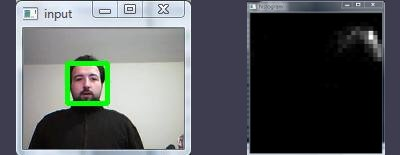
\includegraphics[width=1\textwidth]{face_histo.jpg}
		\end{figure}
	\end{block}
}

\frame{
 \frametitle{Extracting hand from the frames: An example}
  \begin{itemize}
  \item Backproject skin color histogram on whole frame
  \end{itemize}
  \begin{block}{}
  \begin{figure}[!hbtp]
      \centering
      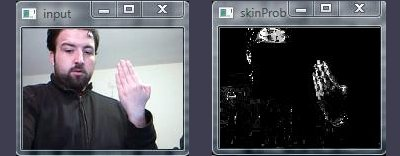
\includegraphics[width=1\textwidth]{skin_rawprob.jpg}
  \end{figure}
  \end{block}
}

\frame{
 \frametitle{Extracting hand from the frames: An example}
  \begin{itemize}
   \item Use erosion \& dilation to reduce the noise and fill up gaps
   \item Extract area of corresponding to the hand
  \end{itemize}
 \begin{block}{}
  \begin{figure}[!hbtp]
      \centering
      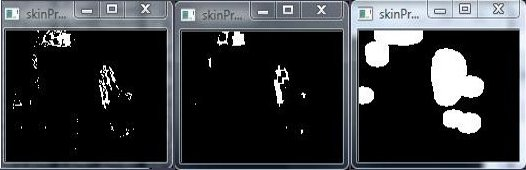
\includegraphics[width=1\textwidth]{skin_eroded_dilated.jpg}
  \end{figure}
  \end{block}
}

\frame{
 \frametitle{Extracting hand from the frames: An example}
   \begin{itemize}
   \item Use more sophisticated erosion \& dilation on hand area
       \begin{itemize}
       \item Retain the hand and remove the background
       \item Resize the area of interest to 70x70
       \end{itemize}
   \end{itemize}
  \begin{block}{} 
   \begin{figure}[!hbtp]
       \centering
       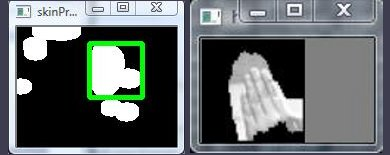
\includegraphics[width=1\textwidth]{blob.jpg}
   \end{figure}
  \end{block}
}
%SILVIA CLASSIFICATION APPROACH_______________________________________________________
\subsection{Classify signs}
\frame{
	\frametitle{Training Data}
	We have used:\\
	\vspace*{5px}
	Grayscale images of \emph{70$\times$70px} with hands at different angles and in different positions and with a black background.\\
	\vspace*{15px}
	\begin{block}{Data -- Example}
		\begin{figure}[!hbtp]
			\centering
			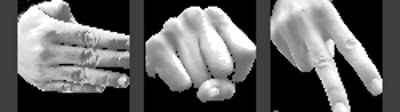
\includegraphics[width=0.9\textwidth]{data.jpg}
		\end{figure}
	\end{block}	
	\fade{\emph{Approximatively 1400 train images per sign.}}
}

\frame{
  \frametitle{Training Features -- PCA}
	The steps for creating the \emph{eigen-hands} are:\\ 
	\vspace*{10px}
	\begin{enumerate}
		\item Extract the mean of the data
		\item Compute the covariance of the data and the eigenvectors of the covariance matrix. For high-dimensional data compute:
		\begin{block}{}
			 \vspace*{5px}
			 \hspace*{45px}\textbf{V} $\rightarrow$ the eigenvectors of: $eigh(\frac{Data\times Data^T}{size(Data))}$\\
			 \vspace*{10px}
			 \hspace*{45px}\textbf{U} $\rightarrow$ the final eigenvectors:  $\frac{Data^T\times V}{norm(Data^T\times V)}$\\
			 \vspace*{5px}
		\end{block}	
		\item Project each training set separately on the eigen-space 		
	\end{enumerate}
}

\frame{
  \frametitle{Training Features -- Gabor wavelets}
	\begin{block}{Gabor wavelets -- Example}
		\begin{figure}[!hbtp]
			\centering
			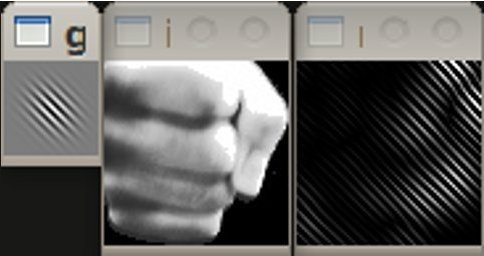
\includegraphics[width=0.9\textwidth]{gabor.jpg}
		\end{figure}
	\end{block}	
}

\frame{
  \frametitle{Train Features -- Gabor wavelets}
	The steps for extracting the features:\\ 
	\vspace*{10px}
	\begin{enumerate}
		\item Create the \emph{Gabor wavelet} using the formula: 
	 \begin{block}{}
		\vspace*{5px}
		\hspace*{45px}\textbf{g(x,y,$\lambda$,$\theta$,$\psi$,$\sigma$,$\gamma$)}= exp(-$\frac{x\prime^2+\gamma^2y\prime^2}{2\sigma^2}$)cos($2\Pi\frac{x\prime}{\lambda}+\psi$)\\
		\vspace*{10px}
		\hspace*{110px}$x\prime$ = x cos$\theta$+y sin$\theta$\\
		\vspace*{5px}
		\hspace*{110px}$y\prime$ = -x sin$\theta$+y cos$\theta$\\	
		\vspace*{5px}
	\end{block}	
		\item Convolve the each image with the resulted wavelet		
		\item Reshape images on a single row (for multiple \emph{Gabor wavelets} concatenate them)
	\end{enumerate}
}

%Nao DESCRIPTION SECTION___________________________________________________________________________________
\subsection{About Nao}
\frame{
	\frametitle{About Nao}
	The third part of the project was to implement movement and communication on \emph{Nao}.\\
	\vspace*{20px}
	\begin{itemize}
		\item \emph{Nao} is sweet (naknak)
		\vspace*{5px}
		\item It has 500MhZ processor
		\vspace*{5px}
		\item It has 3 fingers that move simultaneously
		\vspace*{5px}
		\item Broke his hip 2 times in 6 month
		\vspace*{5px}
		\item It costs 17.500 dollar (16.800k if you buy 5)
		\vspace*{5px}
		\item Additional 3 year maintenance 4.800 dollars
	\end{itemize}
}

%EVALUATION SECTION___________________________________________________________________________________
\section{Evaluation}
\subsection{Experimental Set-up}
\frame{
	\frametitle{Experimental Set-up}
	For gesture recognition we have tried using both the \textbf{SVM} and \textbf{Knn} classifiers.\\
	\vspace*{7px}
	Given the fact that the data is \underline{not aligned} (hands have slightly different positions in the image and different angles) the problem seems to be \underline{too hard for the \textbf{SVM}}.\\
	\vspace*{7px}
	In conclusion we have decided to use \textbf{Knn} for the classification.\\
	\vspace*{20px}
	We have used:\\
	\begin{itemize}
	\item \emph{1522} training examples for the \emph{"paper"} sign
	\item \emph{1641} training examples for the \emph{"rock"} sign 
	\item \emph{1377} training examples for the \emph{"scissors"} sign
	\end{itemize}
}

\subsection{Evaluation Results}
\frame{    
	\frametitle{Evaluation Results}
	\begin{block}{Average errors for each method}
		\begin{tabular}{| c | c | c | c | c | c |}
			\hline\hline\hline
			 	&  	& 	 & 	 &	  &	\\
			\textbf{Size} & \textbf{Method} & \textbf{Rock} & \textbf{Paper} & \textbf{Scissors} & \textbf{Total}\\[7px] 
			\hline\hline\hline
			  70$\times$70 & \emph{PCA} & 0.375 & 0.464 & 0.604 & 0.475\\
			\hline
			  20$\times$20 & \emph{PCA} & 0.381 & 0.477 & 0.570 & 0.470\\
			\hline
			  20$\times$20 & \emph{Gabor} & 0.017 & 0.010 & 0.039 & 0.021\\
			\hline
			  20$\times$20 & \emph{Gabor + PCA} & 0.446 & 0.516 & 0.577 & 0.510\\
			\hline
			  20$\times$20 & \emph{Gabor \& Image} & 0.008 & 0.005 & 0.022 & 0.012\\
		 	\hline
			  20$\times$20 & \emph{(Gabor \& Image)} & 0.331 & 0.483 & 0.549 & 0.447\\
		               & \emph {+ PCA}  &       &	      &       &       \\ 			
			\hline
			  70$\times$70 & \emph{Grayscale} & 0.008 & 0.012 & 0.029 & 0.016\\
			\hline
			  20$\times$20 & \emph{Grayscale} & 0.008 & 0.007 & 0.026 & 0.014\\
			\hline
		\end{tabular}
	\end{block}
}
%CONCLUSION SECTION____________________________________________________________________________________
\section{Conclusions}
\frame{
  \frametitle{Conclusions}
	\begin{itemize}
		\item SVM can handle only very simple cases where only one orientation per
		gesture is allowed 
		\vspace*{8px}
		\item PCA was not strong enough to extract features when all orientations for
		gestures are allowed 
		\vspace*{8px}
		\item KNN works best. Even on raw images
		\vspace*{8px}
		\item When not perfect images are used (slightly different positions and different angles) results
		tend to drop
		\vspace*{8px}
		\item More reliable results were obtained by enriching our training sets with examples of hands extracted by skin-detection with the method described above
	\end{itemize}
}

\end{document}


